
\section{Device Manufacturing}

\subsection{PDMS Channel Fabrication}
\par The device microchannels were fabricated by pouring PDMS (polydimethysiloxane) over a silicon wafer master mold. Through photolithography, a master mold was created by patterning a silicon wafer with SU-8 photoresist in  a process known as soft lithography. A 6"x6" 20,000 DPI negative transparency mask was ordered from CAD/Art Services Inc. with the emulsion face down. A general process flow is depicted in figure \ref{fig:soft_lithography_flow}.


\subsection*{SU-8 Master Mold}

\par Before photolithography, silicon wafers were cleaned in a Piranha bath ( 98\% sulfuric acid, get pirahna def) for 15 minutes and then rinsed in DI (deionized) water, and dipped in BOE solution (get BOE def) for 5 minutes and then rinsed in DI water. The wafers were then washed and dried in the SRD (spin rinse dry) machine before baking the wafers at 205$^\circ$ for 10 minutes on a hot plate to dehydrate the wafers, and allowed to cool for 10 minutes. 

\begin{figure}[h]
    \centering
    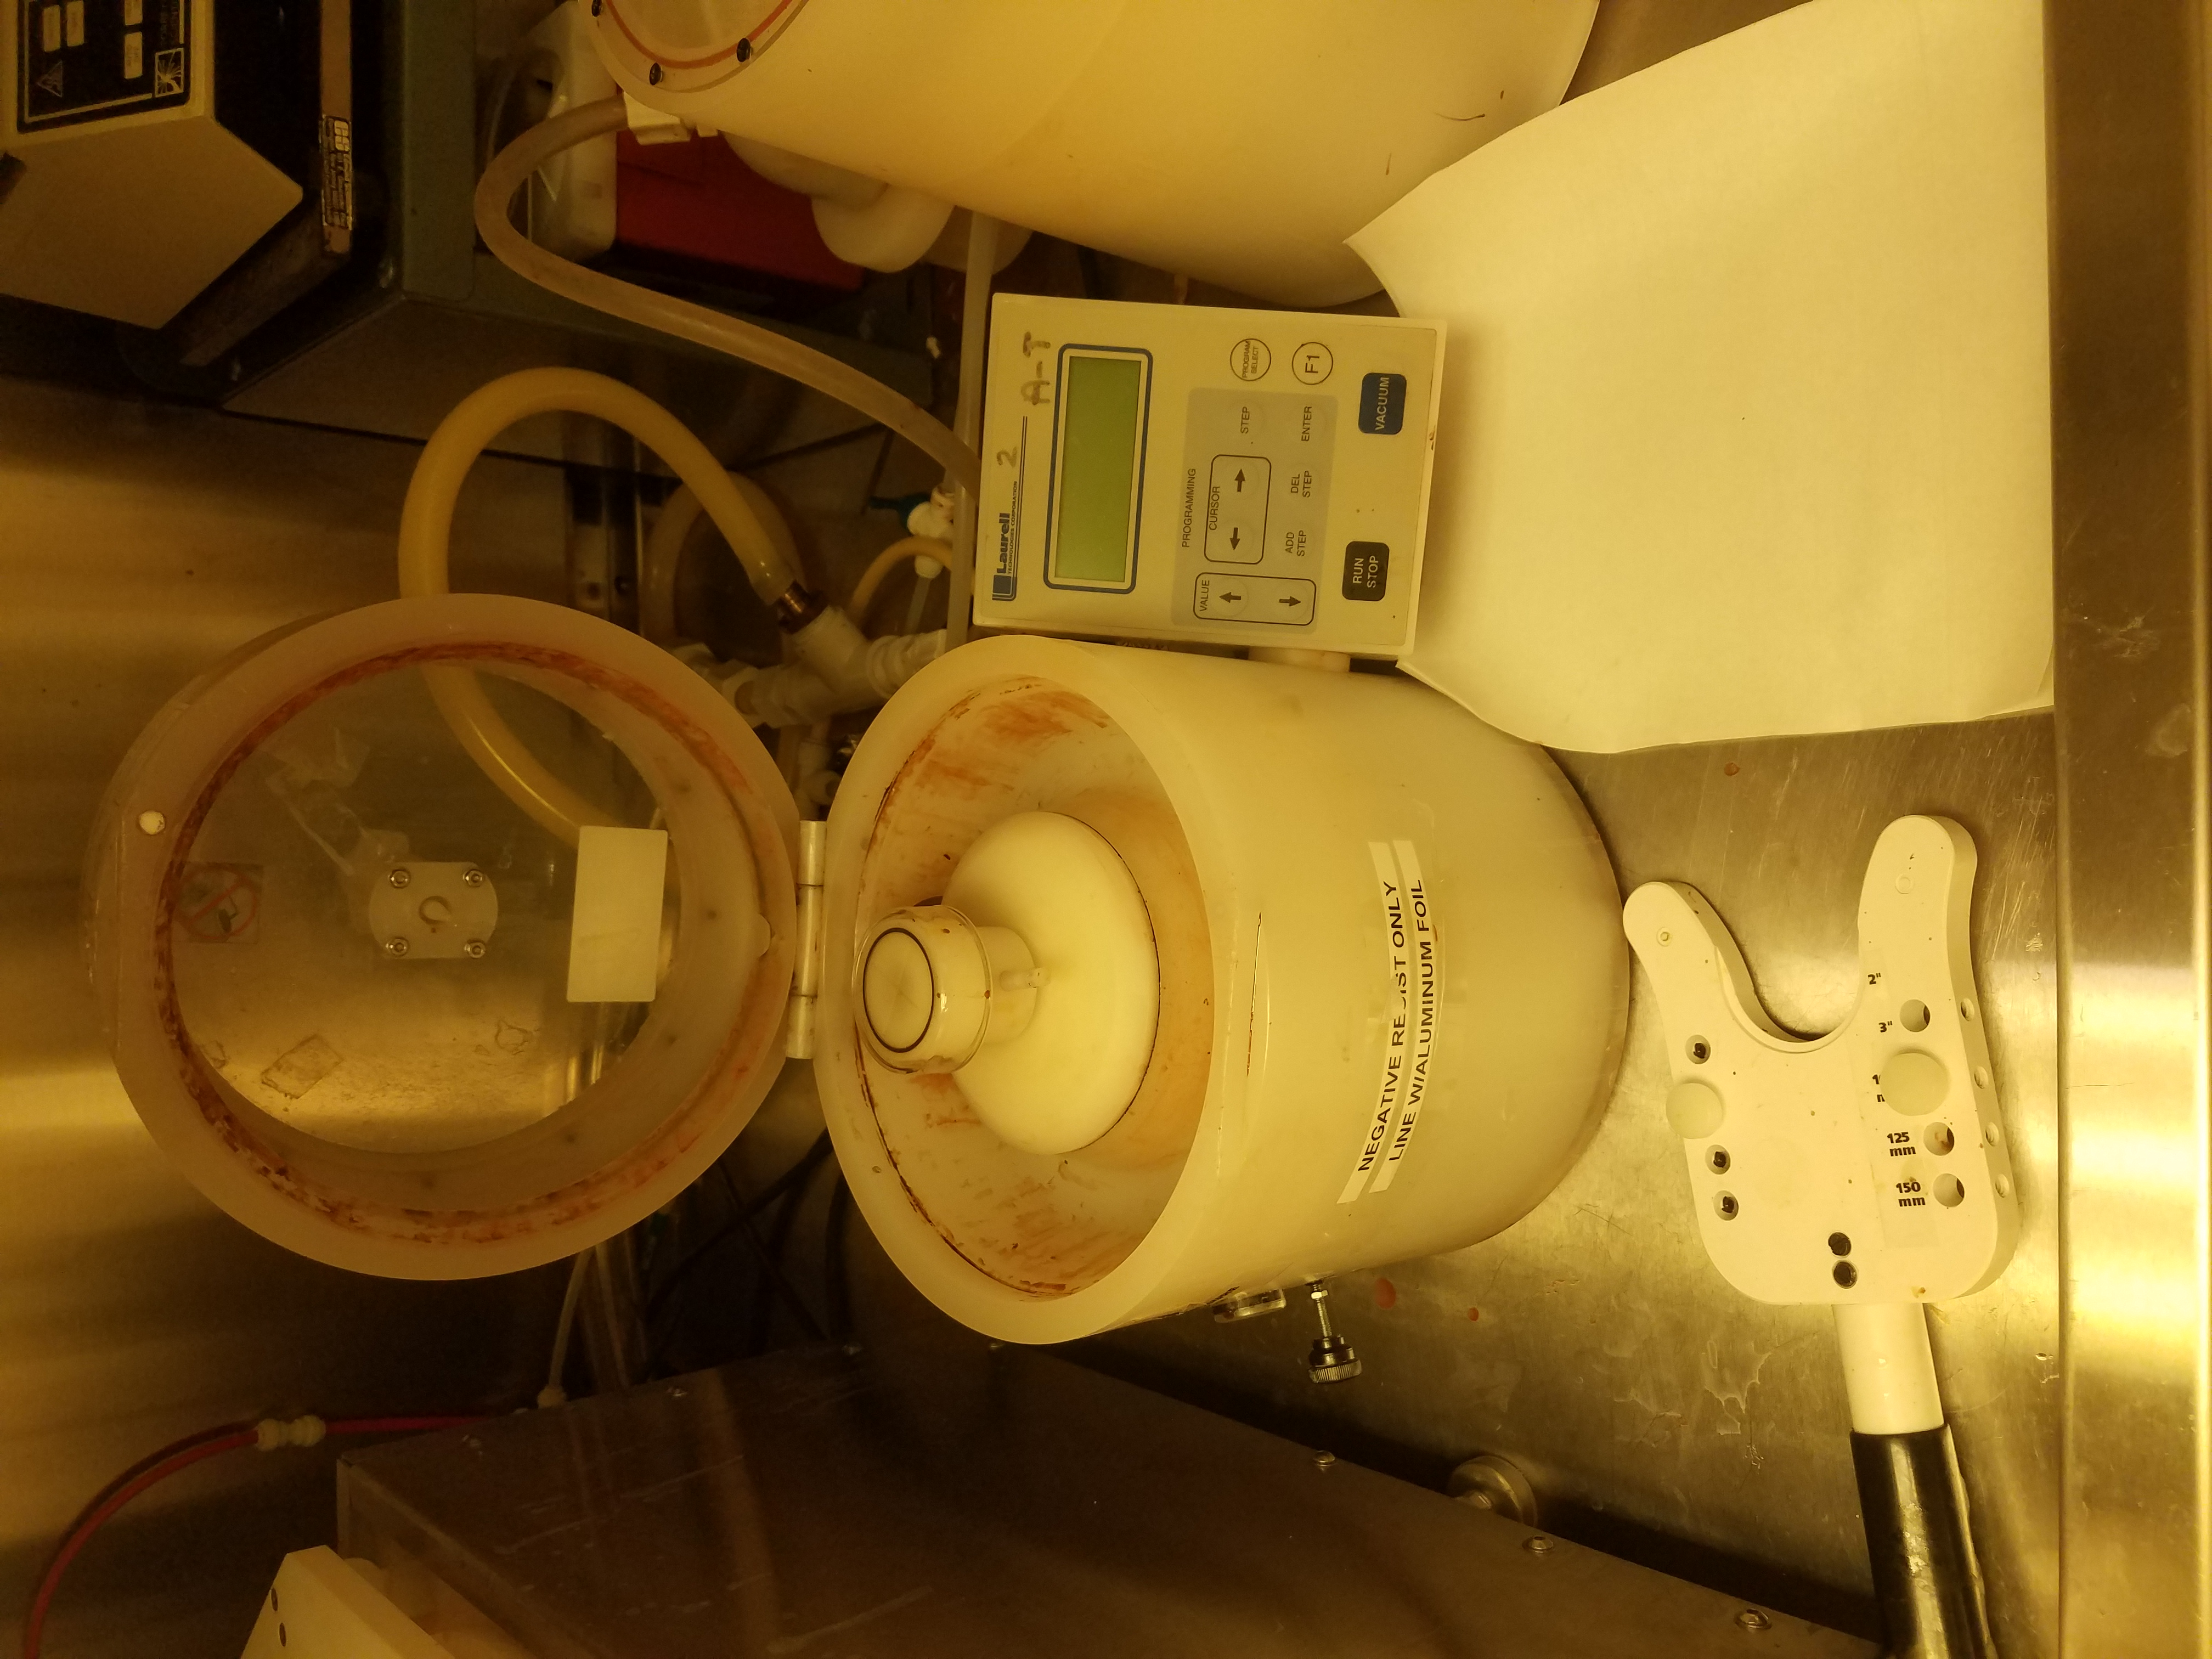
\includegraphics[width=0.7\textwidth]{images/resist_spinner_open.jpg}
    \caption{Laurel Technologiers ws-400 spin coater}
    \label{fig:spin_coater}
\end{figure}

\par The wafers were coated with SU-8 (a negative tone photoresist) on a spin coater (Laurel Technologies, ws-400; figure \ref{fig:spin_coater}). The spin coater rotates at a series of specific angular velocities in order to coat the wafer with the desired thickness of photoresist. About 4 mL of SU-8 2007 (\#07110769, MicroChem) was placed on the center of the wafer and then spun for 400 RPM for 20 seconds to disperse the SU-8, and then at 1500 RPM for 35 seconds to spread the photoresist to a 10 $\mu$m thickness. After spin-coating, the wafer was soft-baked at 85$^\circ$C for 3 minutes and allowed to cool for 4 minutes.

\begin{figure}[h]
    \centering
    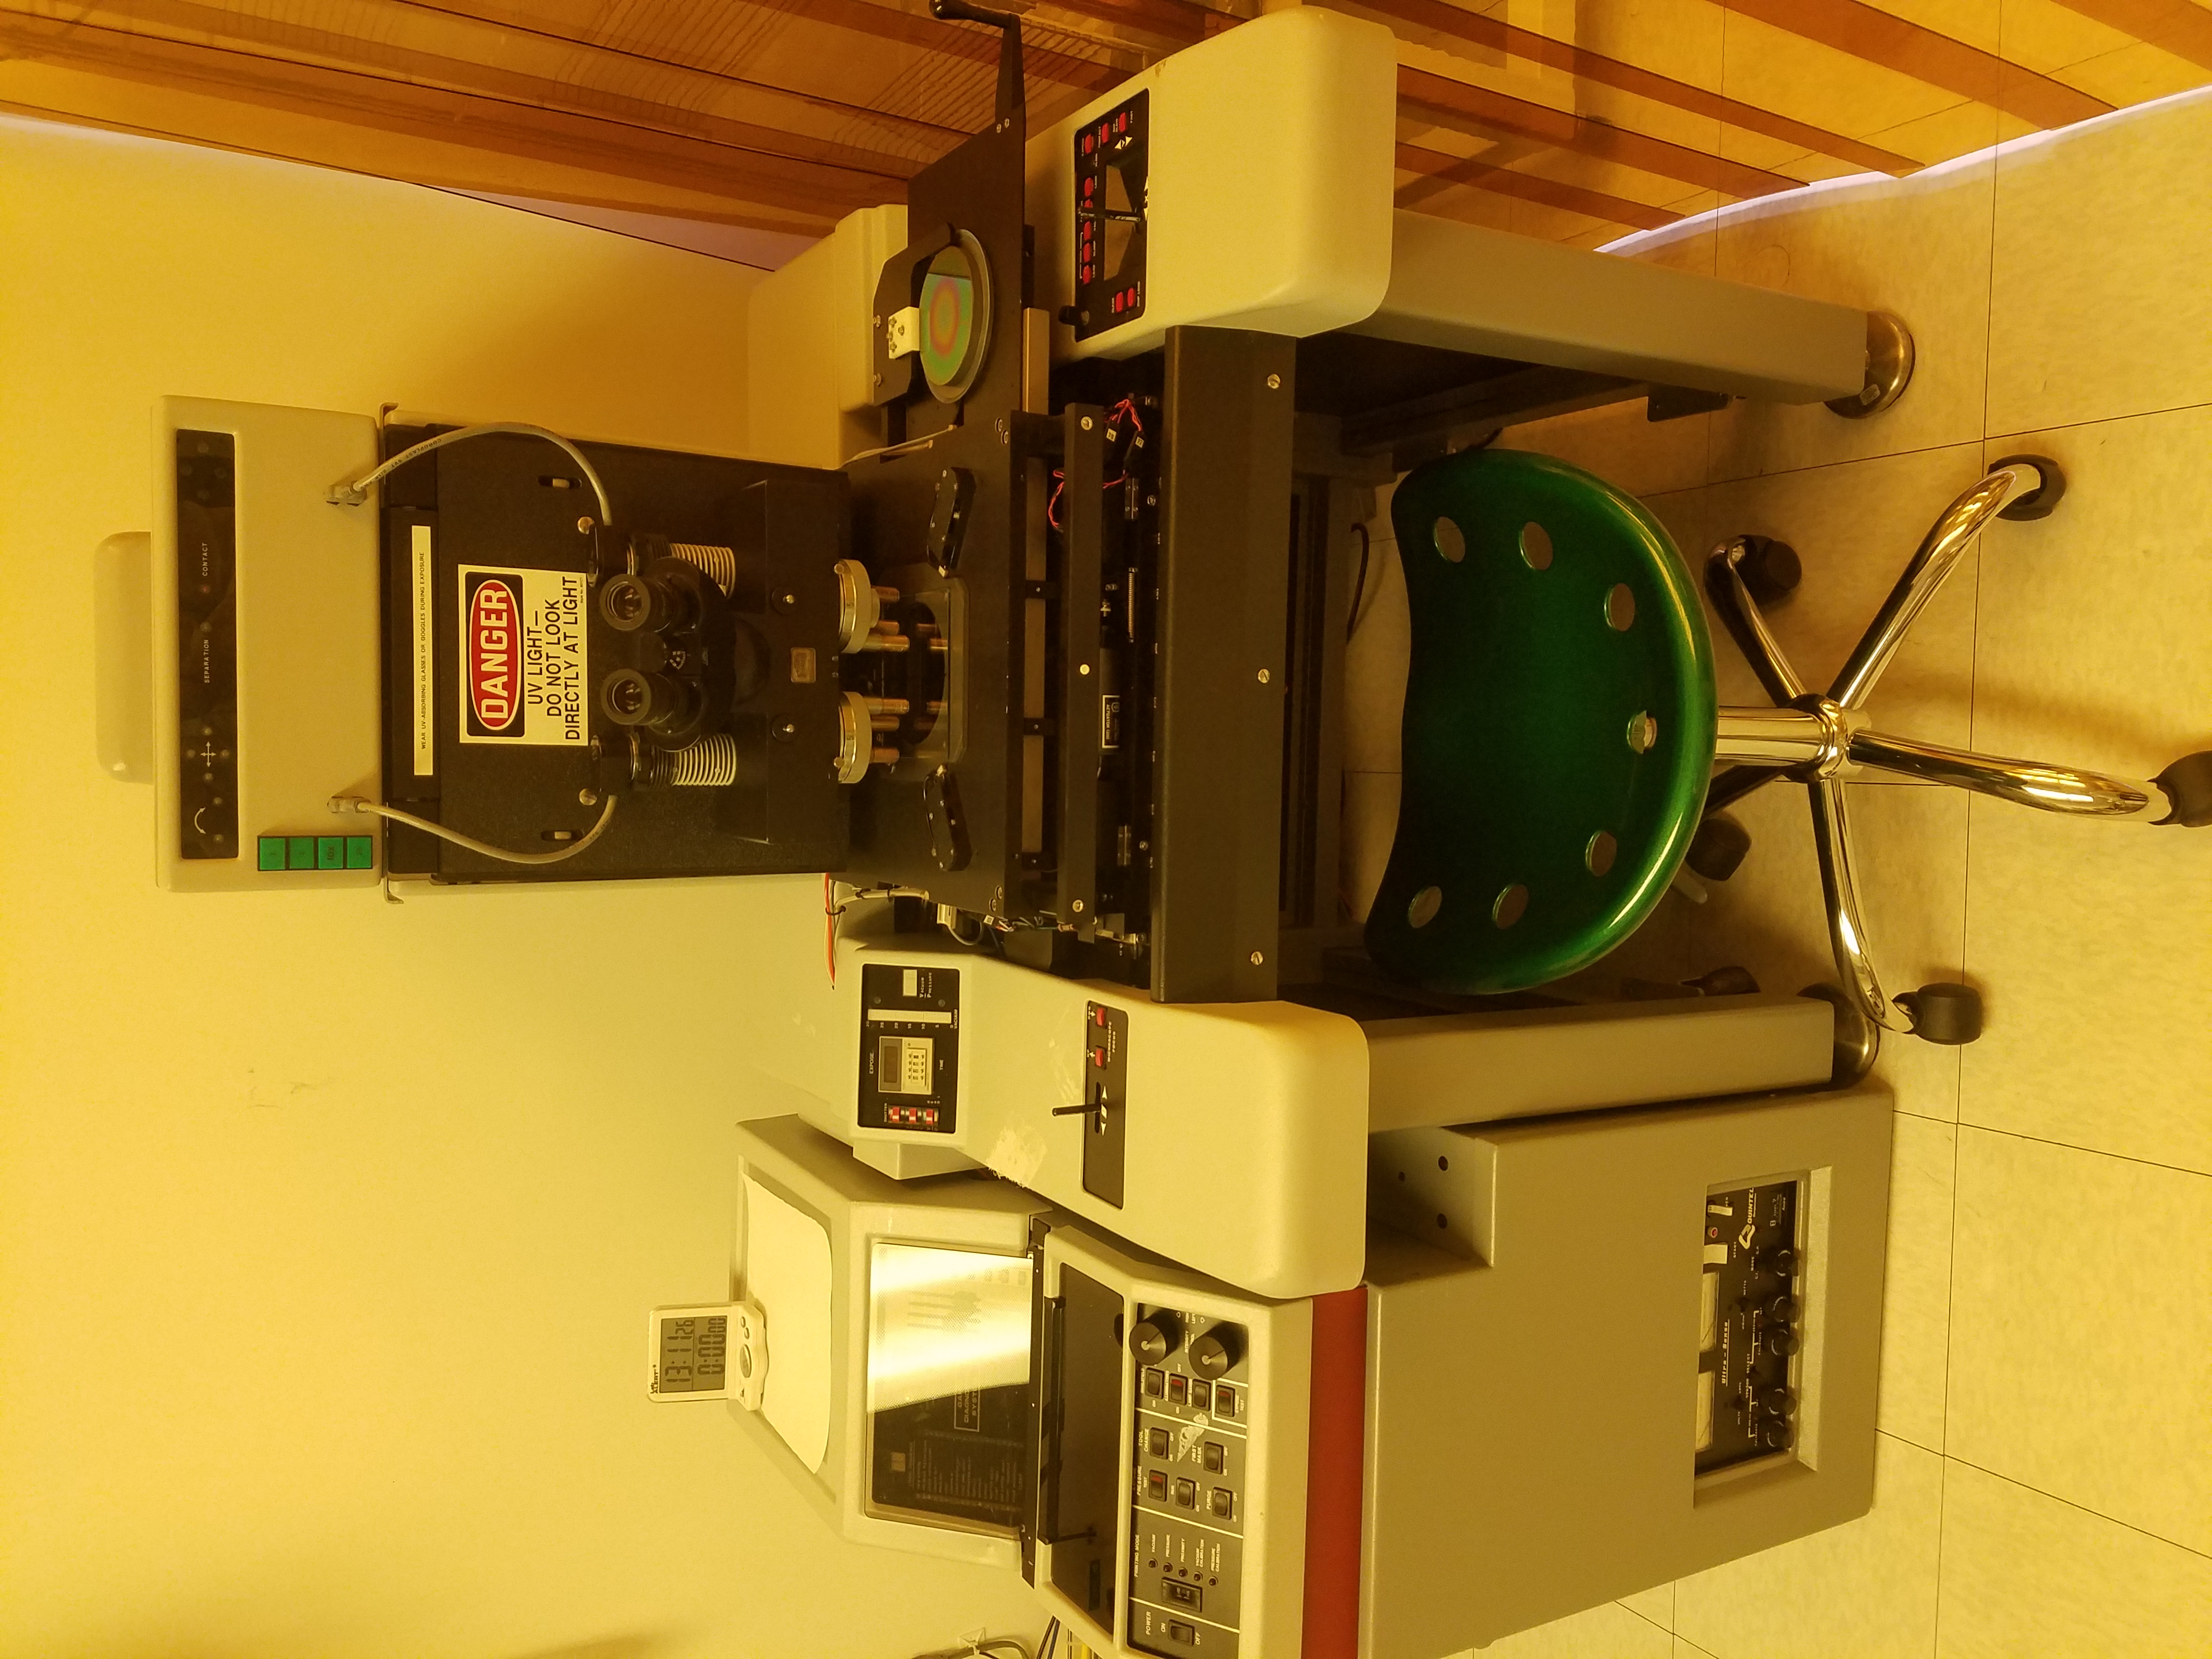
\includegraphics[angle=-90,origin=c,width=0.65\textwidth]{images/aligner.jpg}
    \caption{Caption}
    \label{fig:my_label}
\end{figure}

\par The photolithography process was completed using the Cannon PLA-501FA mask aligner (figure \ref{fig:mask_aligner}). With the transparency mask centered over the wafer and the 365 nm glass-transparency??? in place, UV light was applied to the photoresist for 14 seconds with a total exposure of 140 mJ/cm$^2$. The wafer was then baked at 85 $^\circ$C for 4 minutes with a 10 minute cool down. 

\par The wafer was then developed in propylene glycol monomethyl ether acetate (SU-8 developer, MicroChem) in order to remove the non-exposed SU-8 from the wafer. The wafer was placed in the SU-8 developer for 3 minutes. The wafer was then hard baked for 15 minutes at 210 $^\circ$C. 

The detailed procedure steps are provided in appendix \ref{app: su-8_photolith}.

\subsection*{Soft Lithography}
\par The polydimethylsiloxane (PDMS) for soft lithography was obtained by purchasing a Dow Corning 184 Sylgard kit through Ellsworth adhesives. The kit comes with a base and a curing agent that cross links the PDMS and increases the polymer's stiffness. The PDMS was prepared by mixing the base and the curing agent with a 10:1 ration. The mixture was then degassed under vacuum until the PDMS was clear and free of bubbles (figure \ref{fig: pdms_vacuum}). The PDMS was then poured directly onto the SU-8 master mold until the PDMS covered the wafer with approximately 1/4" depth. The PDMS was cured by baking in an oven for at least an hour at 65 $^\circ$. The PDMS chips were cut from the master mold with a scapel and peeled off the wafer. Using a ?? hole puncher, the microchannel inlets and outlets were punched with the device side down. 

\par The finished product is a PDMS chip with the desired microchannel dimensions molded into the polymer surface. The procedure steps for soft lithography are provided in appendix \ref{app: soft_litho}.


\subsection{Electrode Fabrication: Lift-off Process}
\par The device electrodes were fabricated onto a glass substrate using the lift-off process (section \ref{sec: lift_off}). The process utilized a 6"x6", 20,000 DPI transparency mask ordered from CAD/art services Inc. A flow chart of the overall process is depicted in figure \ref{fig: lift-off_flow_chart}.

\subsection*{Photolithography}
\par Glass wafers were prepared for the lift-off process by cleaning the wafers in a pirahna bath (pirahna def??) for 15 minutes and rinsing in DI water, and then a 1 minute dip in BOE (BOE definition???) and rinsing in DI before running the wafers through the SRD (SRD definition???). The wafers were then dehydrated by baking on a hot plate for 10 minutes at 200 $^\circ$C and then allowed to cool down fro five minutes. 

\par The wafers were coated with ma-N1420 negative-tone photoresist on a spin coater (Laurel technologies, ws-400; \ref{fig: spin_coater}). The ma-N1420 photoresist is advantageous for the lift-off process since the developed photoresist has an undercut profile and the cross-linked photoresist is durable in contrast to the "soft" positive photoresist. Before application of the ma-N1420 a primer (primer definition???) is dispersed and then spun onto the wafer at 3000 RPM for 30??? seconds. Ma-N1420 is then dispersed onto the glass wafer, but before spinning, ensure that the photoresist spreads to all edges of the wafer. The photoresist was spun at 2000 RPM for 35??? seconds with a target of 2.5 micron thickness. The wafers were then soft-baked on a hotplate at 120 $^\circ$C for 3 minutes to increase stability. 

\par The photolithography process was completed using the Cannon PLA-501FA mask aligner. The galss wafer was placed in the aligner with a black tape backing in order to prevent light scattering and absorb radiation, and the transparency was centered over the wafer. UV light was applied to the wafer for 30 seconds for a total of 450 mJ/cm$^2$. 

\par The wafer was then developed for 60-90 seconds in something?? based developer (ma-D 533/3) and then rinsed in DI water. At this step, it is critical to examine the wafer under a microscope to ensure the photoresist is entirely removed from the substrate where the electrode is desired and that the electrode edges are sharp. If not, develop for another 10 seconds and reexamine. 

\par After the photoresist is fully developed, the wafer was flood-exposed (i.e. no transparency) in order to improve stability. The photoresist was exposed 3 times for 40 seconds with a five minute rest between each exposure for a total of 1800 mJ/cm$^2$ of exposure. Finally, the wafers were baked on the hotplate with a ramping temperature from 60 $^\circ$C to 100 $^\circ$C for 10 minutes, and then allowed to cool for 10 minutes. 

\subsection*{Metal Deposition}

\par To deposit the electrode metals onto the developed-photoresist wafer, the AGS reactive ion etcher, CrC-150 chrome sputterer, and the Denton Desk V sputtering system were used to clean and sputter chromium and gold. The target metal deposition consists of three layers: a 175 \si{\angstrom} thick base chromium layer to facilitate adhesion of the electrode to glass, a 180 nm thick gold layer as the main conductor in the electrode, and a 42 \si{\angstrom} thick layer of chromium that will oxidize to an inert finish (figure ???).

\par To prepare the photoresist-developed wafer for metal deposition, the wafers were exposed to an oxygen plasma to volatilize and remove organic residues. The wafer was placed under vacuum in the AGS RIE system and exposed to an oxygen plasma for 30 seconds (fig. ??). The CrC-150 sputtering system was then used to deposit 175 \si{\angstrom} of chromium at a rate of 250 \si{\angstrom} per minute for 30 seconds. Using the Denton Desk 5, 180 nm of gold was deposited at a rate of 180 \si{\angstrom} per minute for 10 minutes. A final 42 \si{\angstrom} layer of chromium was deposited with the CrC-150 with a rate of 250 \si{\angstrom} per minute for 10 seconds. 

\par During the transition between sputtering systems, the wafers were kept under vacuum in order to keep them clean, and in the case for chromium depositions, to reduce the formation of chromium oxide which can significantly impair chromium-gold adhesion.

\subsection*{Lift Off}

The final step of the electrode fabrication process was to remove the photoresist with the undesired metal depositions. The wafers were submerged in Microposit remover 1165 for five days under constant agitation. To increase the speed of lift off, the solution can be heated to 65$^\circ$C.

\subsection{Device Assembly: Plasma Bonding and Alignment}
\par To assemble the PDMS chip containing the microfluidic channels to the electrodes on the glass substrate, the components were plasma bonded to create a water-tight seal that still permitted optical viewing. The PDMS and the galss electrode substrate were placed device-side up in the Cal Poly Microfabrication Lab's PDC-32G plasma cleaner. After pumping the plasma cleaner down to a vacuum, the device was exposed to an atmospheric plasma for 10 seconds.  

\par After plasma activation, a drop of ethanol was place don the PDMS surface before placing the PDMS onto the electrode substrate in order to create a liquid float barrier to that will prevent permanent binding for $\sim$5 minutes. The electrodes and PDMS microchannels were aligned by hand with a microscope set at 20X magnification for visual feedback. After proper alignment, the device was baked in an oven at 65$^\circ$C for an hour. 


\section{Device Implementation}


\section[IS Software]{Impedance Spectroscope Software: LabVIEW Programming}
\par LabVIEW was used to interface with the NI-5421 function generator and the NI-5124 oscilloscope to package the circuit model, data acquisition, and data analysis into a impedance spectroscope program. The LabVIEW language was chosen due to the ease of connecting to the National Instrument hardware and the rapid development cycle. The program specifications include interfacing with the NI-hardware to run an impedance spectroscopy experiment, the ability to control the sweeping frequencies, the ability to switch circuit topologies, the ability to automatically run tests at specified intervals, the implementation of a data saving system that records the users settings for the experiment as well as the impedance spectroscopy results, and a way to view and compare data.

\par The LabVIEW program was designed with an event-driven state machine architecture and is diagrammed in figure \ref{fig:event_driven_state_machine_architecture}. A state machine is a common LabVIEW coding pattern where the program exists as a set of states. Depending on user input or calculations, each state leads to a subsequent state that can potentially lead to a large network of modular decision making states. For the impedance spectroscope, the state machine is simple with most states leading to an idle state that continues to wait for user input. The state machine lives inside an event structure that listens for specific user interface (UI) interactions that triggers an event that runs code and can specify the next state in the state machine. After a specified amount of time passes without an event triggering, the time out event will trigger and run the state machine.    

\begin{figure}[h]
    \centering
    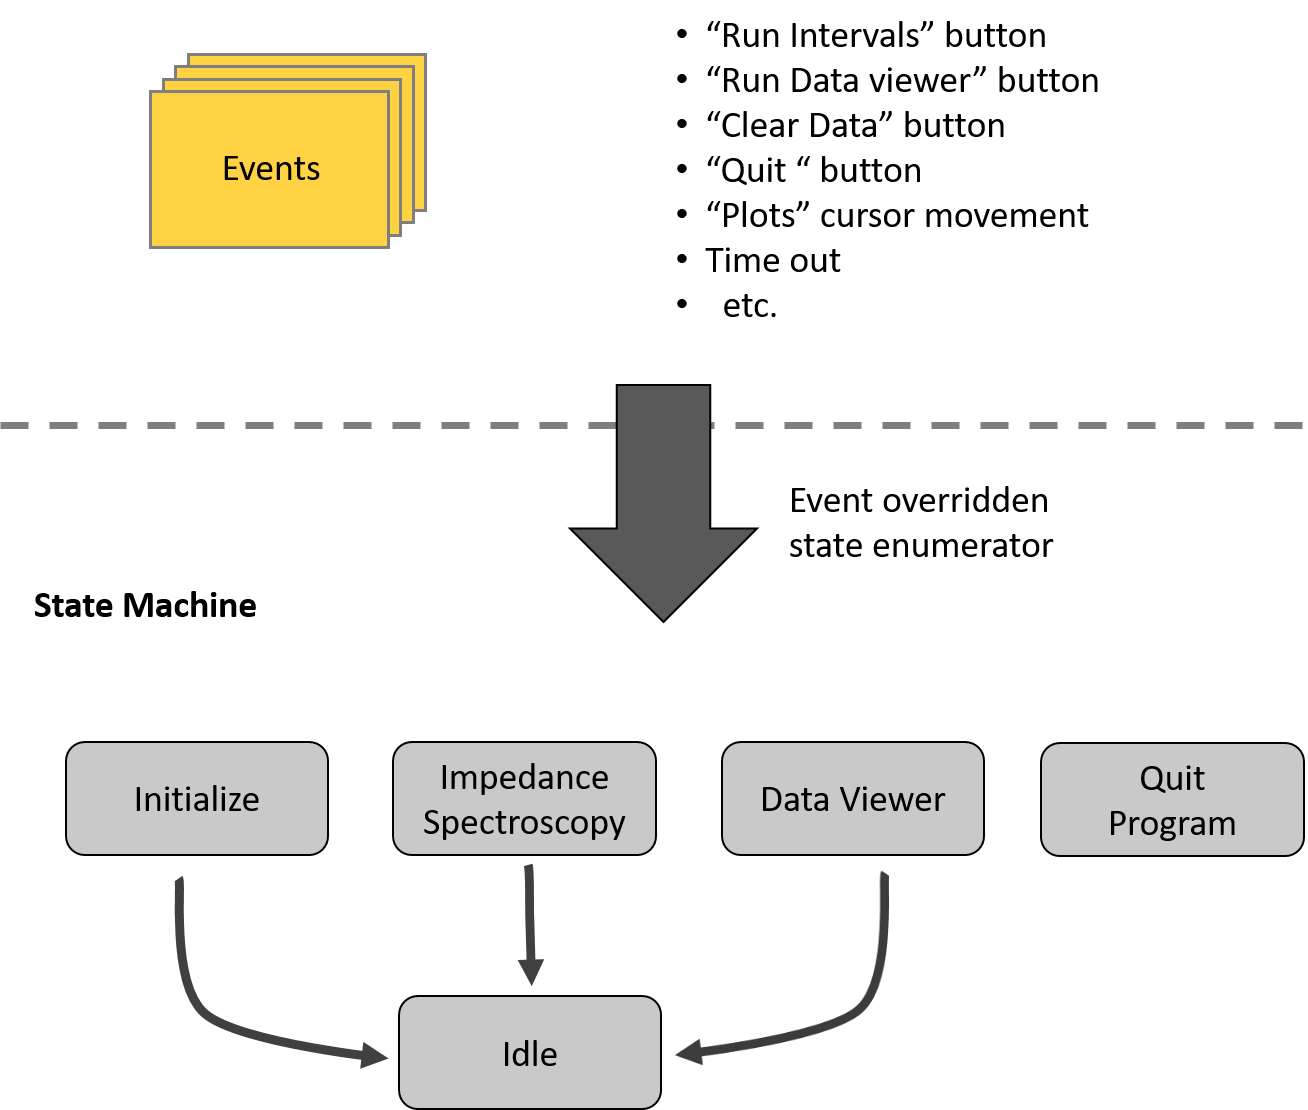
\includegraphics[width=\textwidth]{images/program_overview.png}
    \caption{The event-driven state machine architecture used for the impedance spectroscope LabVIEW program. Events override the state of the state machine that runs inside the time out event.}
    \label{fig:event_driven_state_machine_architecture}
\end{figure}

\par The event driven state machine architecture will allow for a responsive UI that can adapt outside of the state machine architecture while maintaining the modularity of a state machine with safe program initialization and exit. 